\chapter{The Piston Engine}

Most cars,  airplanes,  and chainsaws get their power from burning hydrocarbons in a 
combustion chamber.   We say they have \newterm{internal combustion engines}.   There are many types of internal combustion engines: jet engines, rotary engines, diesel engines, and more.  In this chapter, we are 
going to explain how one type,  piston engines, work.   Most cars have piston engines.

Most piston engines burn gasoline,  which is a blend of liquid hydrocarbons.  Hydrocarbons are molecules made of hydrogen and carbon (and maybe a little oxygen).  In the presence of oxygen and heat,  hydrocarbons burn --- the carbon combines with oxygen to become $CO_2$, and the hydrogen combines with oxygen to become $H_2O$.  In the process, heat is released, which causes the gases in the cylinder to create a lot of pressure on the piston.


\section{Parts of the Engine}

The engine block is a big hunk of metal.  There are cylindrical holes bored into the engine block.  A piston can slide up and down the cylinder.  There are two valves in the wall of the cylinder:  
\begin{itemize}
\item Before the burn, one valve opens to let ethanol and air into the cylinder.
\item After the burn,  the other valve opens to let the exhaust out.
\end{itemize}

There is also a spark plug, which creates the spark that triggers the burn.

As you give the engine more gas,  the cylinder does more frequent burns.  When the engine is just idling,  the cylinder fires about 9 times per second.  When you depress the gas pedal all the way down,  it is more like 40 times per second.

The cylinder has a rod that connects it to the crank shaft. As the pistons move back and forth,  the crank shaft turns around and around.  Sometimes a piston is pushing the crankshaft, and sometimes the crank shaft is pushing or pulling the piston.  All the cylinders share one crank shaft.

How many cylinders does a car have?  Nearly all car models have between 3 and 8 cylinders. The opening of the valve and the firing of the spark plugs are timed so that cylinders all do their burns 
at different times. This makes the total power delivered to the crank shaft smoother.


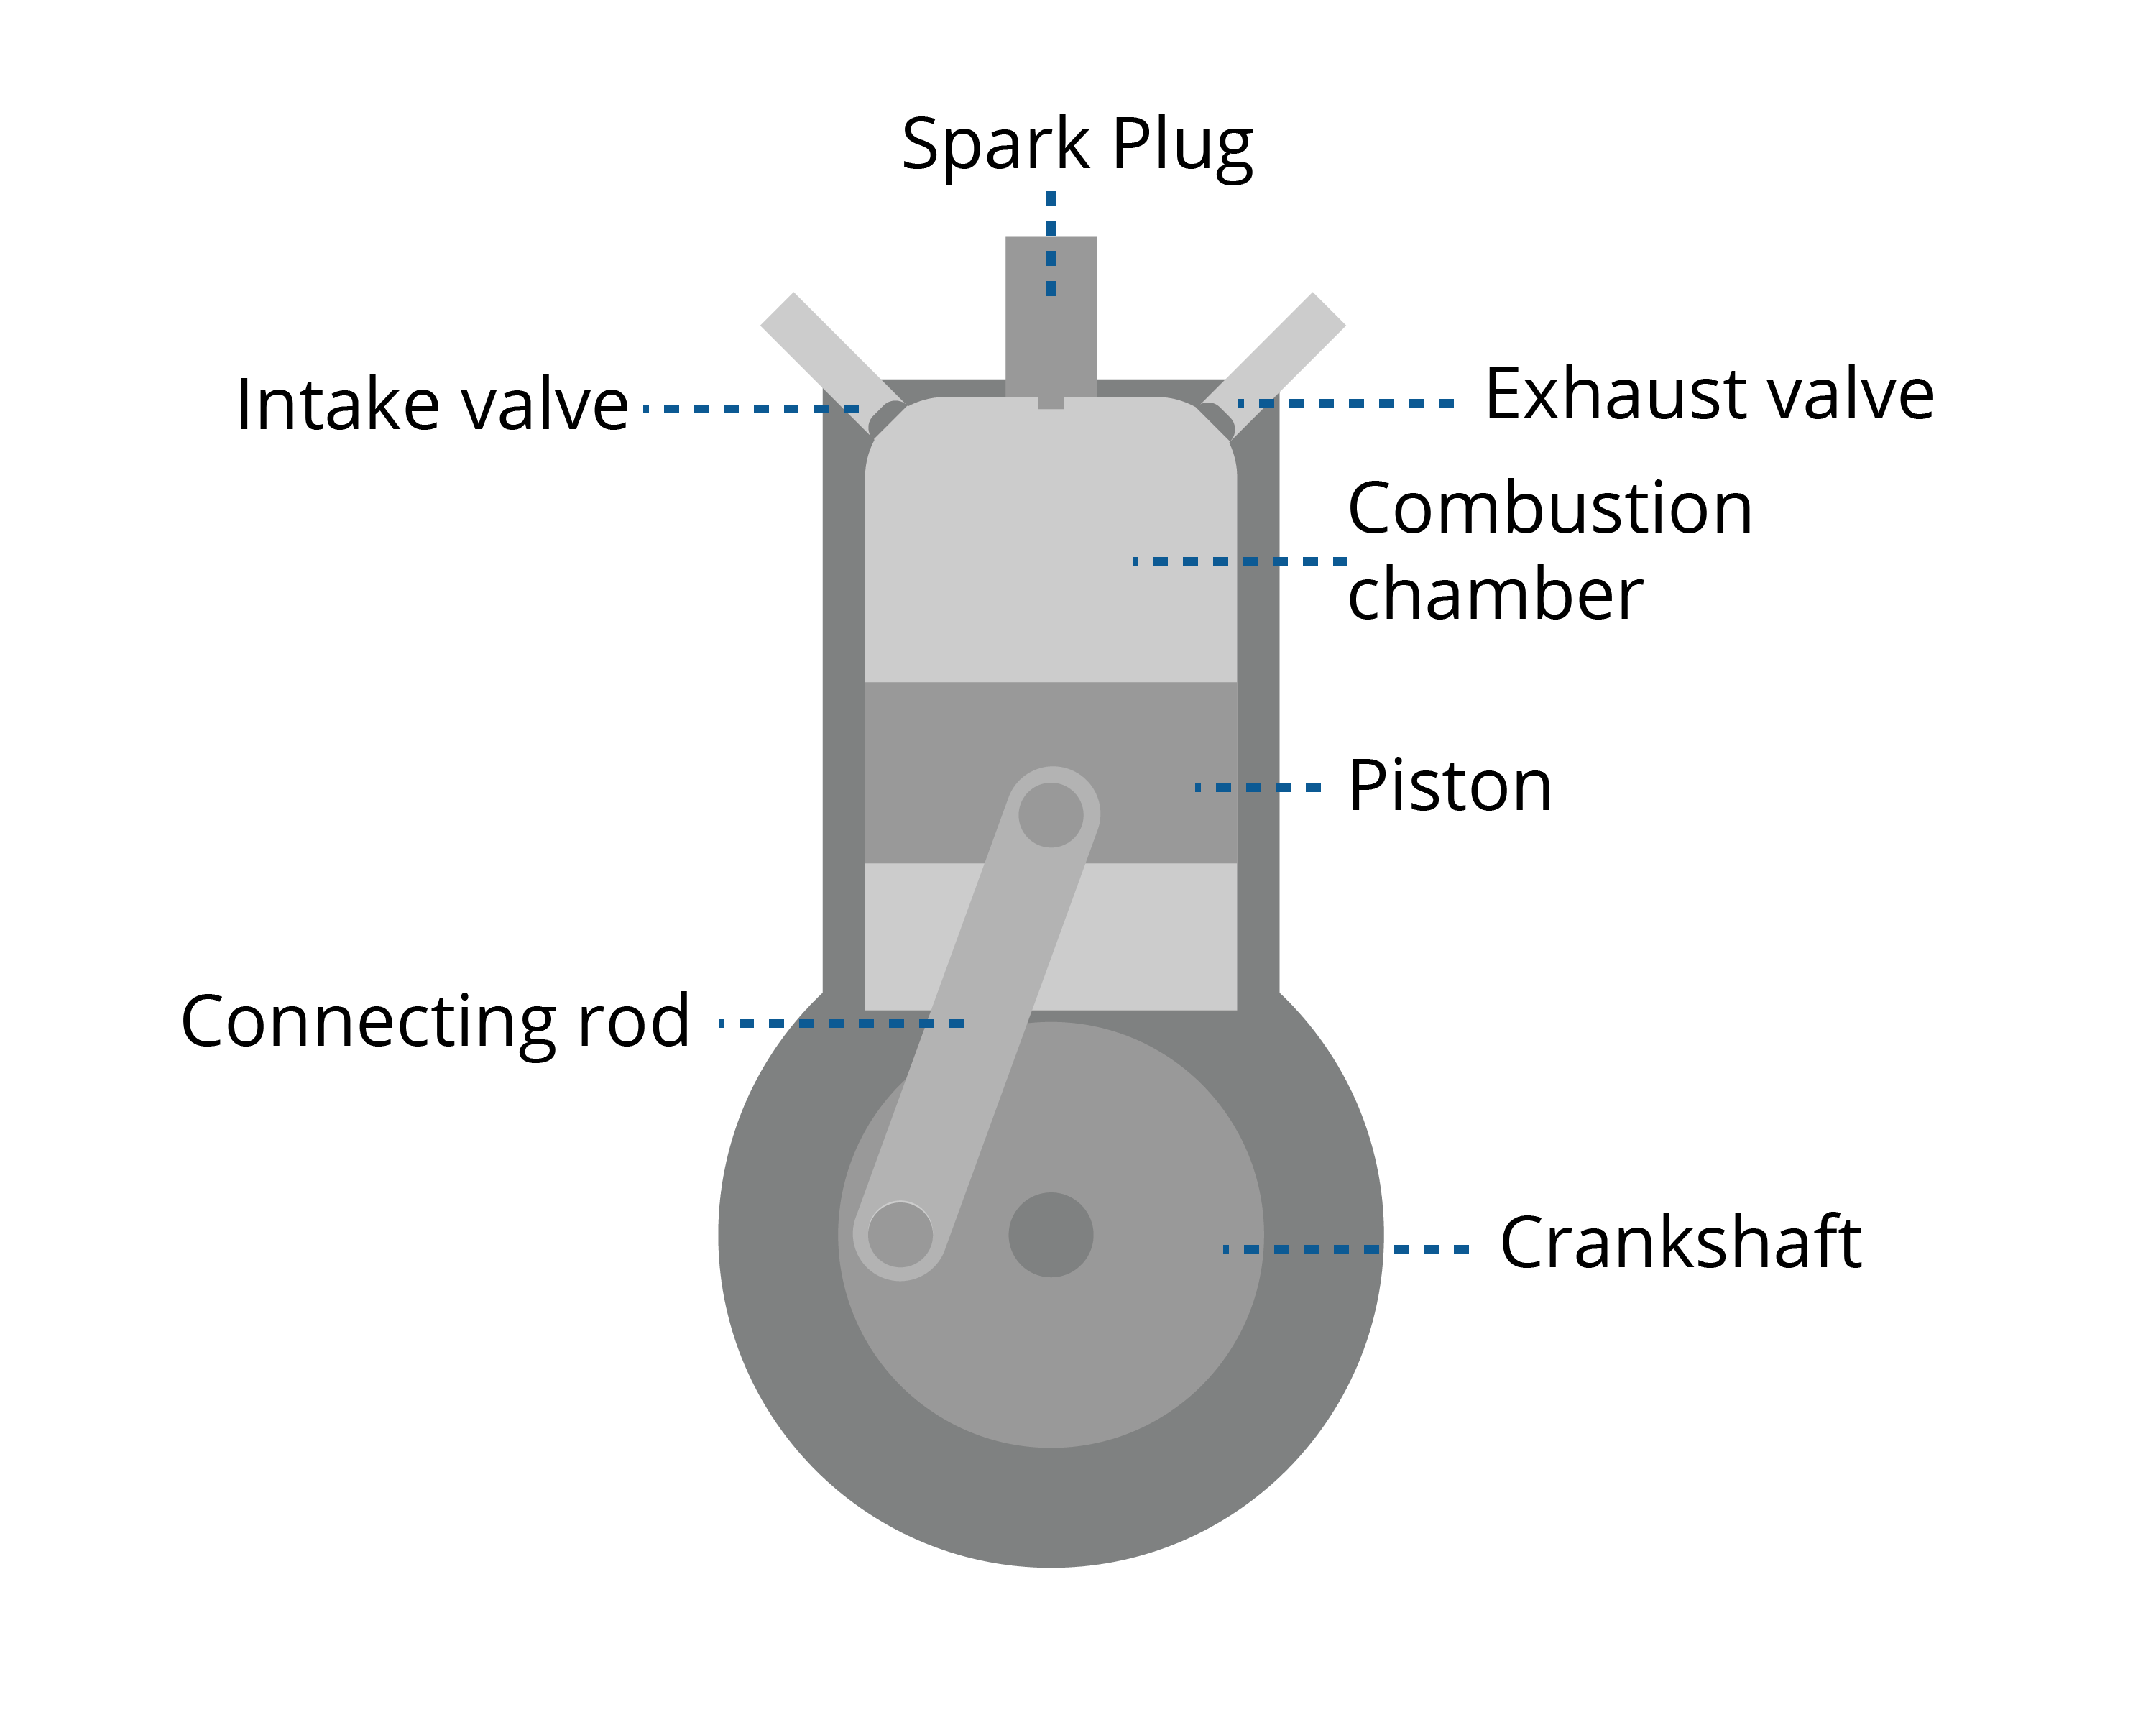
\includegraphics[width=0.75\textwidth]{engine-08.png}


\section{The Four-Stroke Process}

Cars have four-stroke engines --- this means for every two rotations of the crank shaft,  each cylinder fires once.  Smaller engines, like those in chainsaws,  are often two-stroke engines --- every cylinder fires every time the crank shaft rotates.  For now,  let's focus on four-stroke engines.




Here is the cycle of a single cylinder:
\begin{itemize}

\item As the drive shaft turns,  it pulls the piston down.  The intake valve opens and lets the gas/air mixture into the combustion chamber.

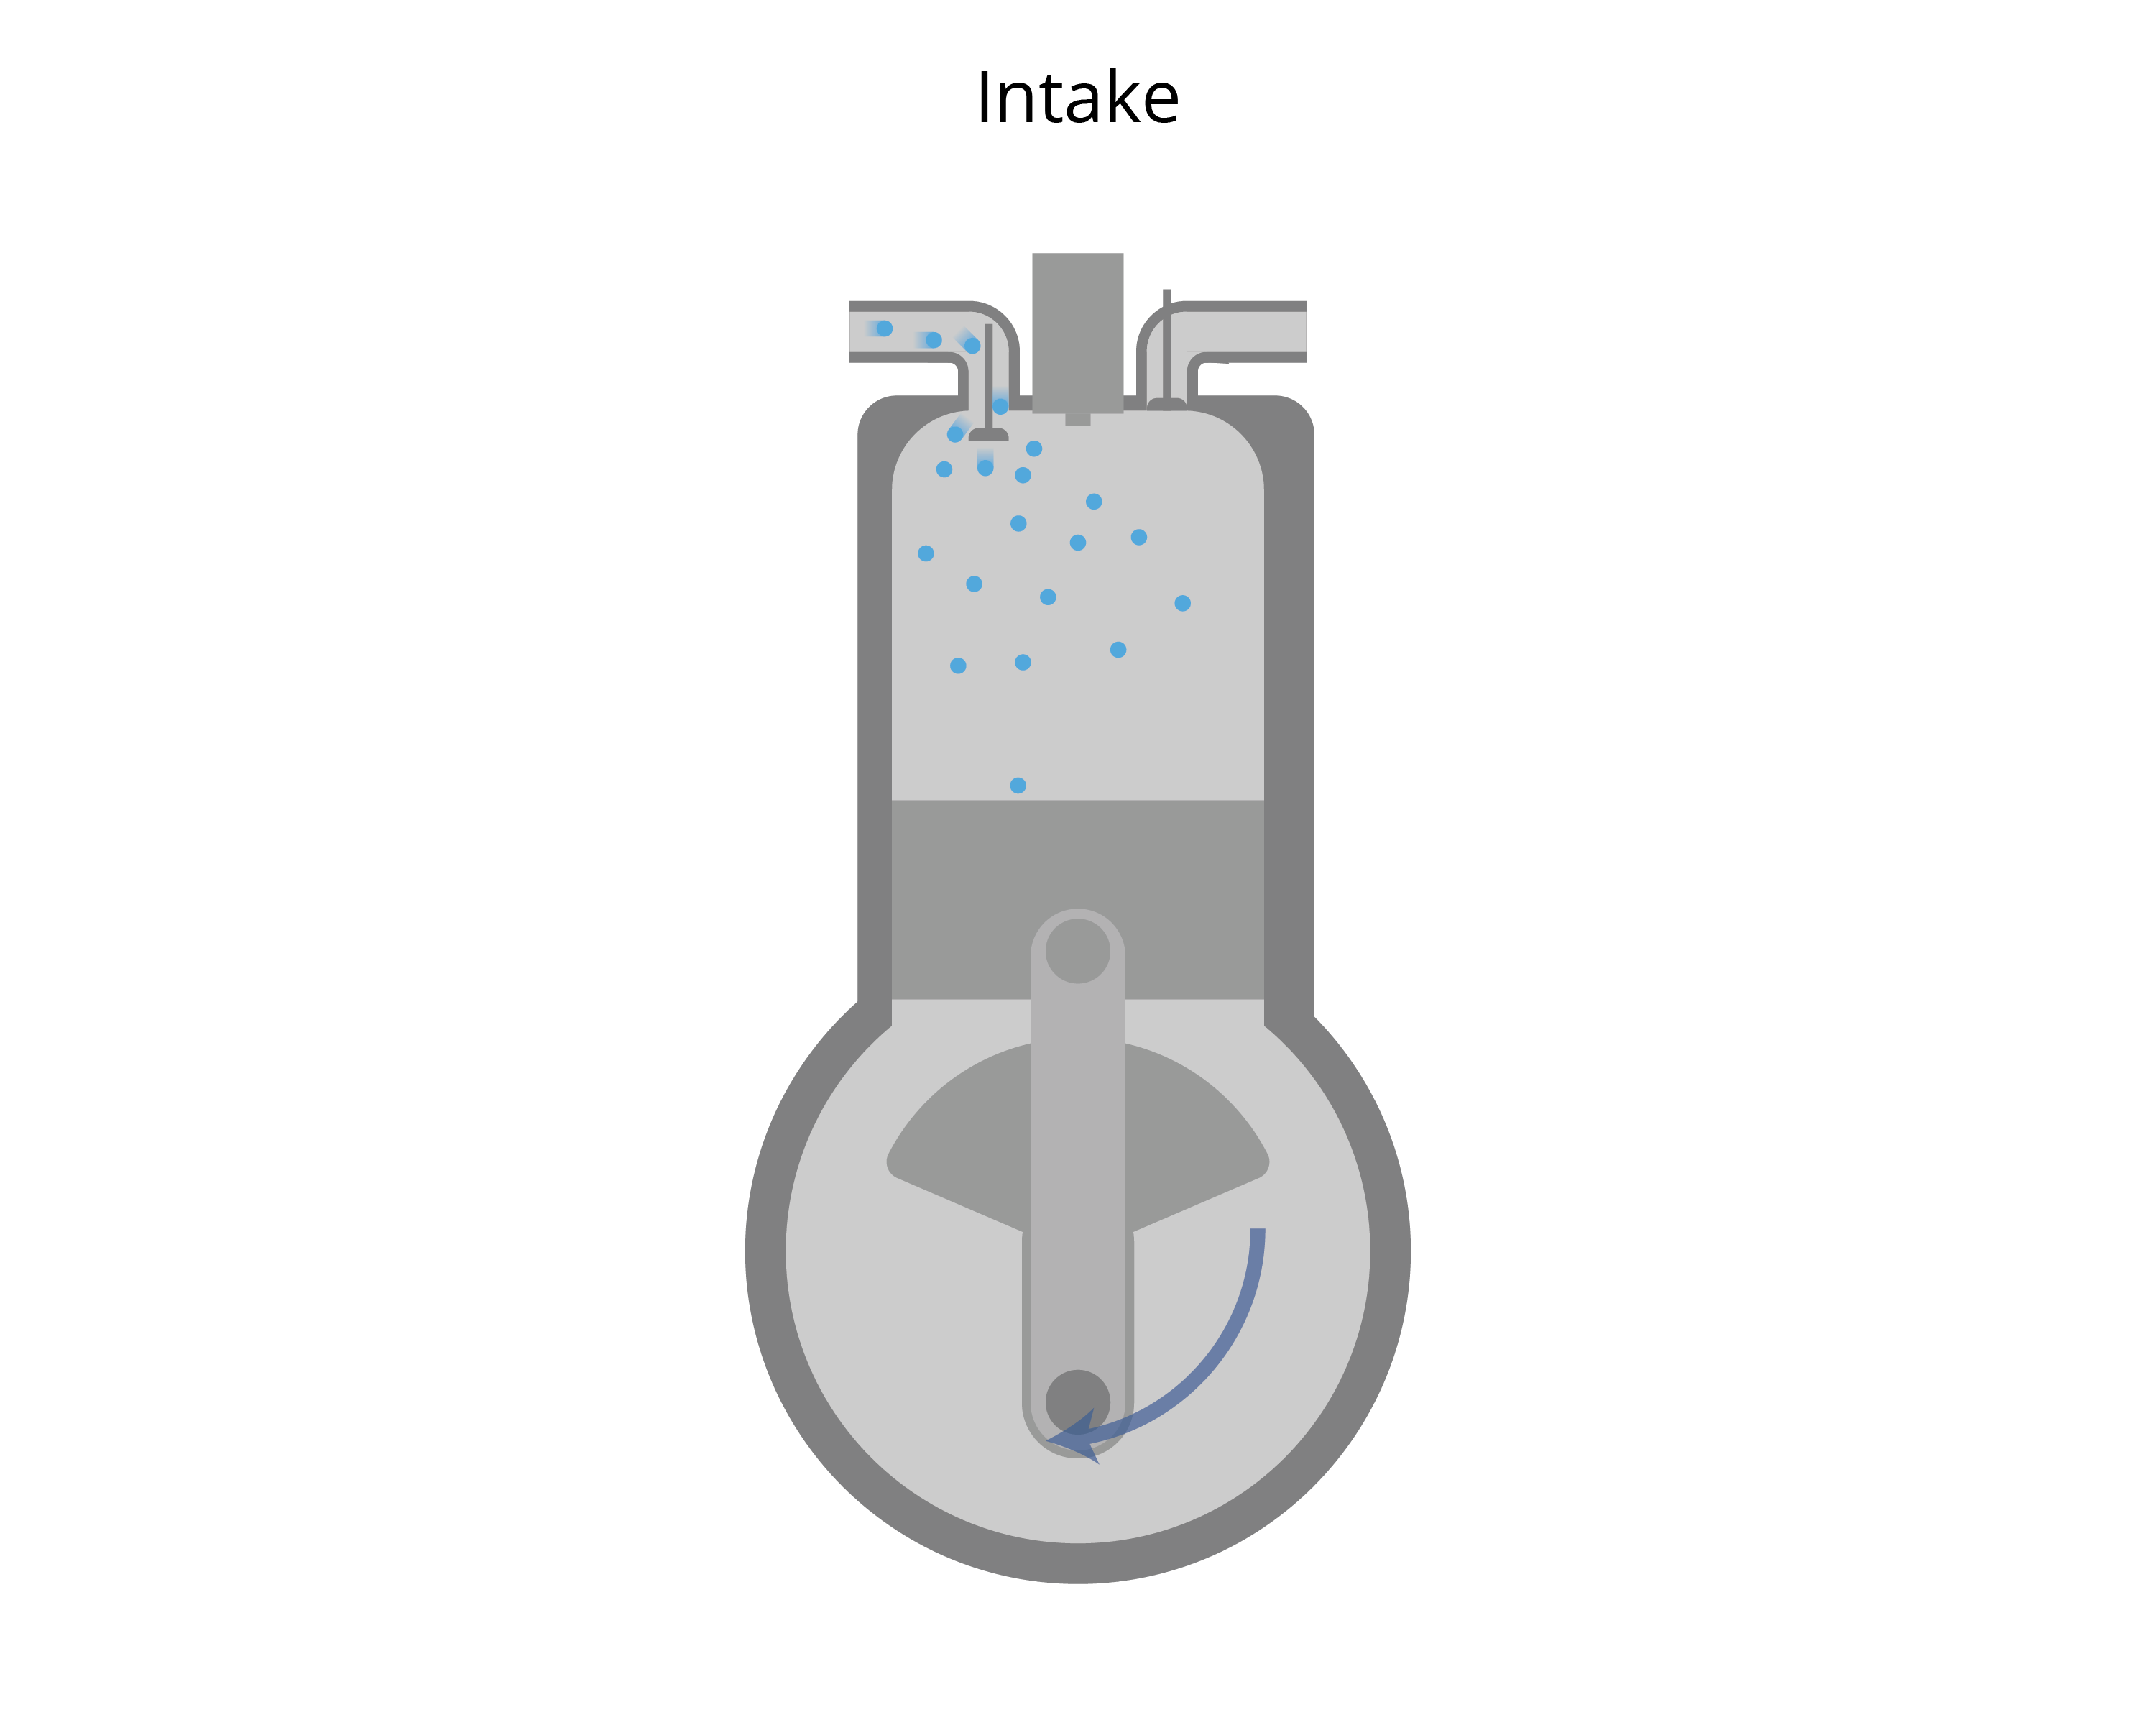
\includegraphics[width=0.75\textwidth]{engine-09.png}

\item As the piston reaches the bottom of the stroke,  the intake valve closes.
\item Now, the crank shaft starts to push the piston up, compressing the gas and oxygen.

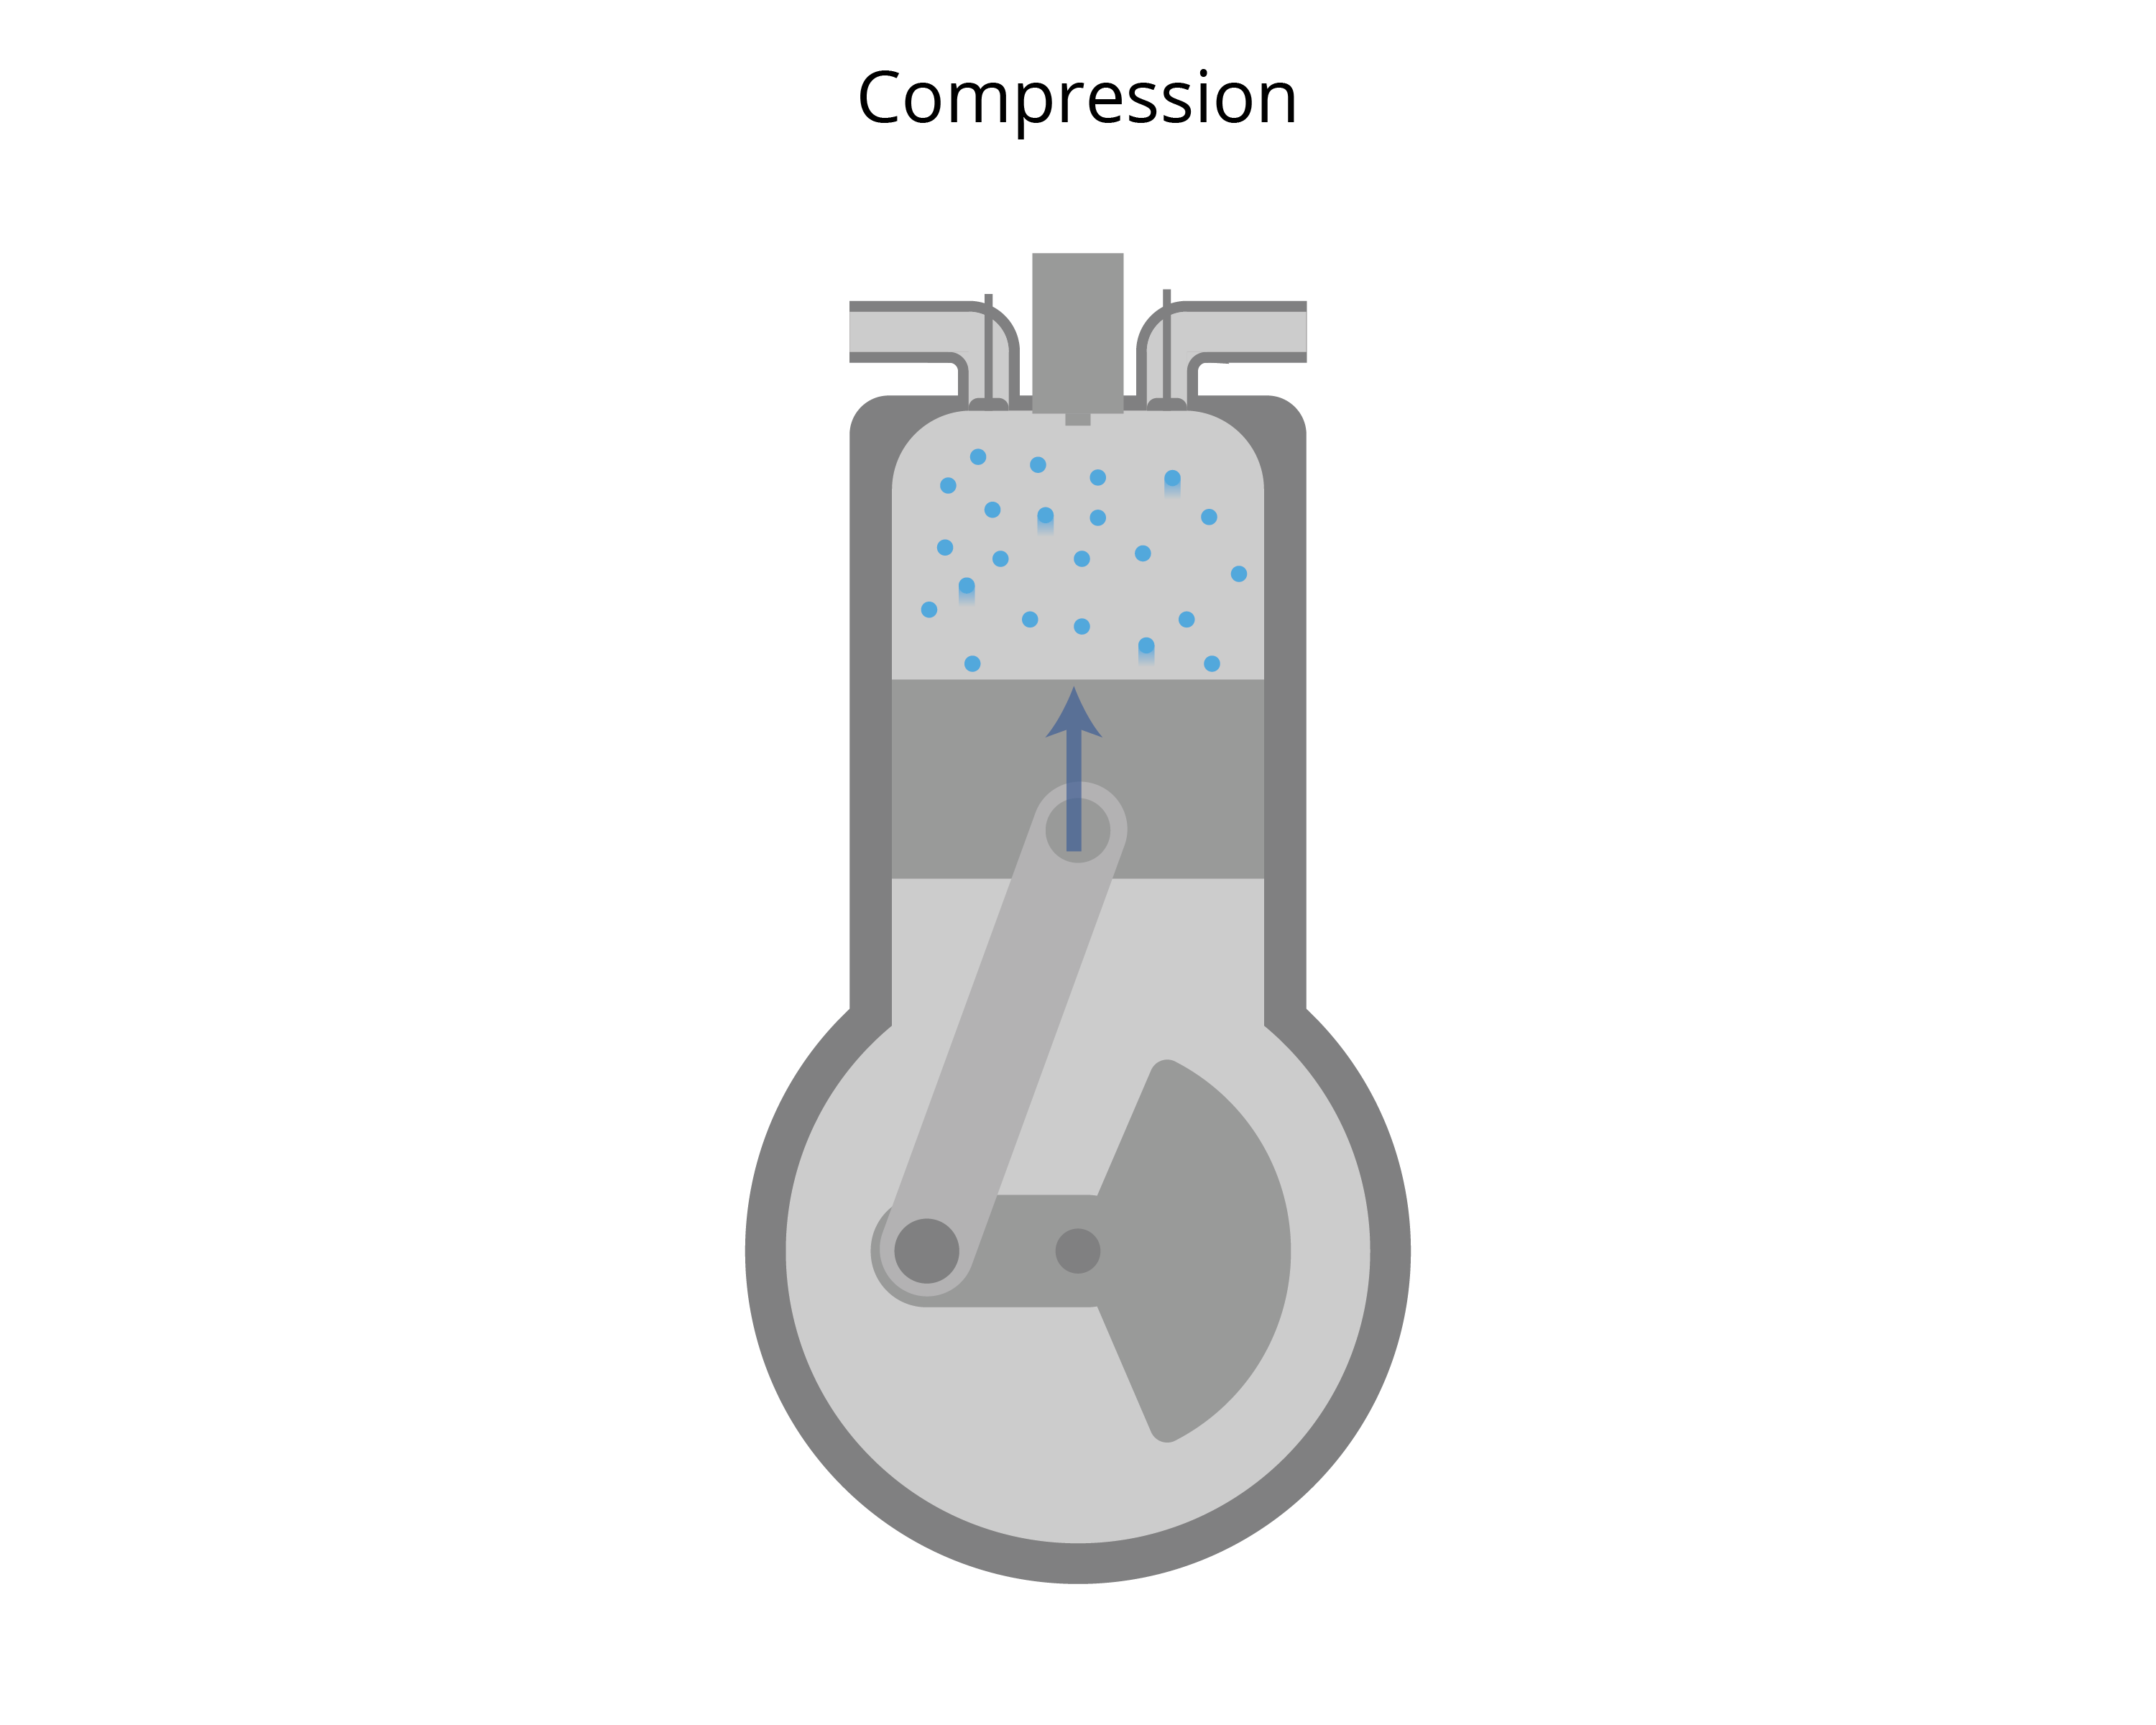
\includegraphics[width=0.75\textwidth]{engine-10.png}

\item As the piston reaches the top of its stroke,  the spark plug creates a spark.  The fuel and oxygen burn quickly.  The cool liquid fuel becomes hot carbon dioxide and water vapor.

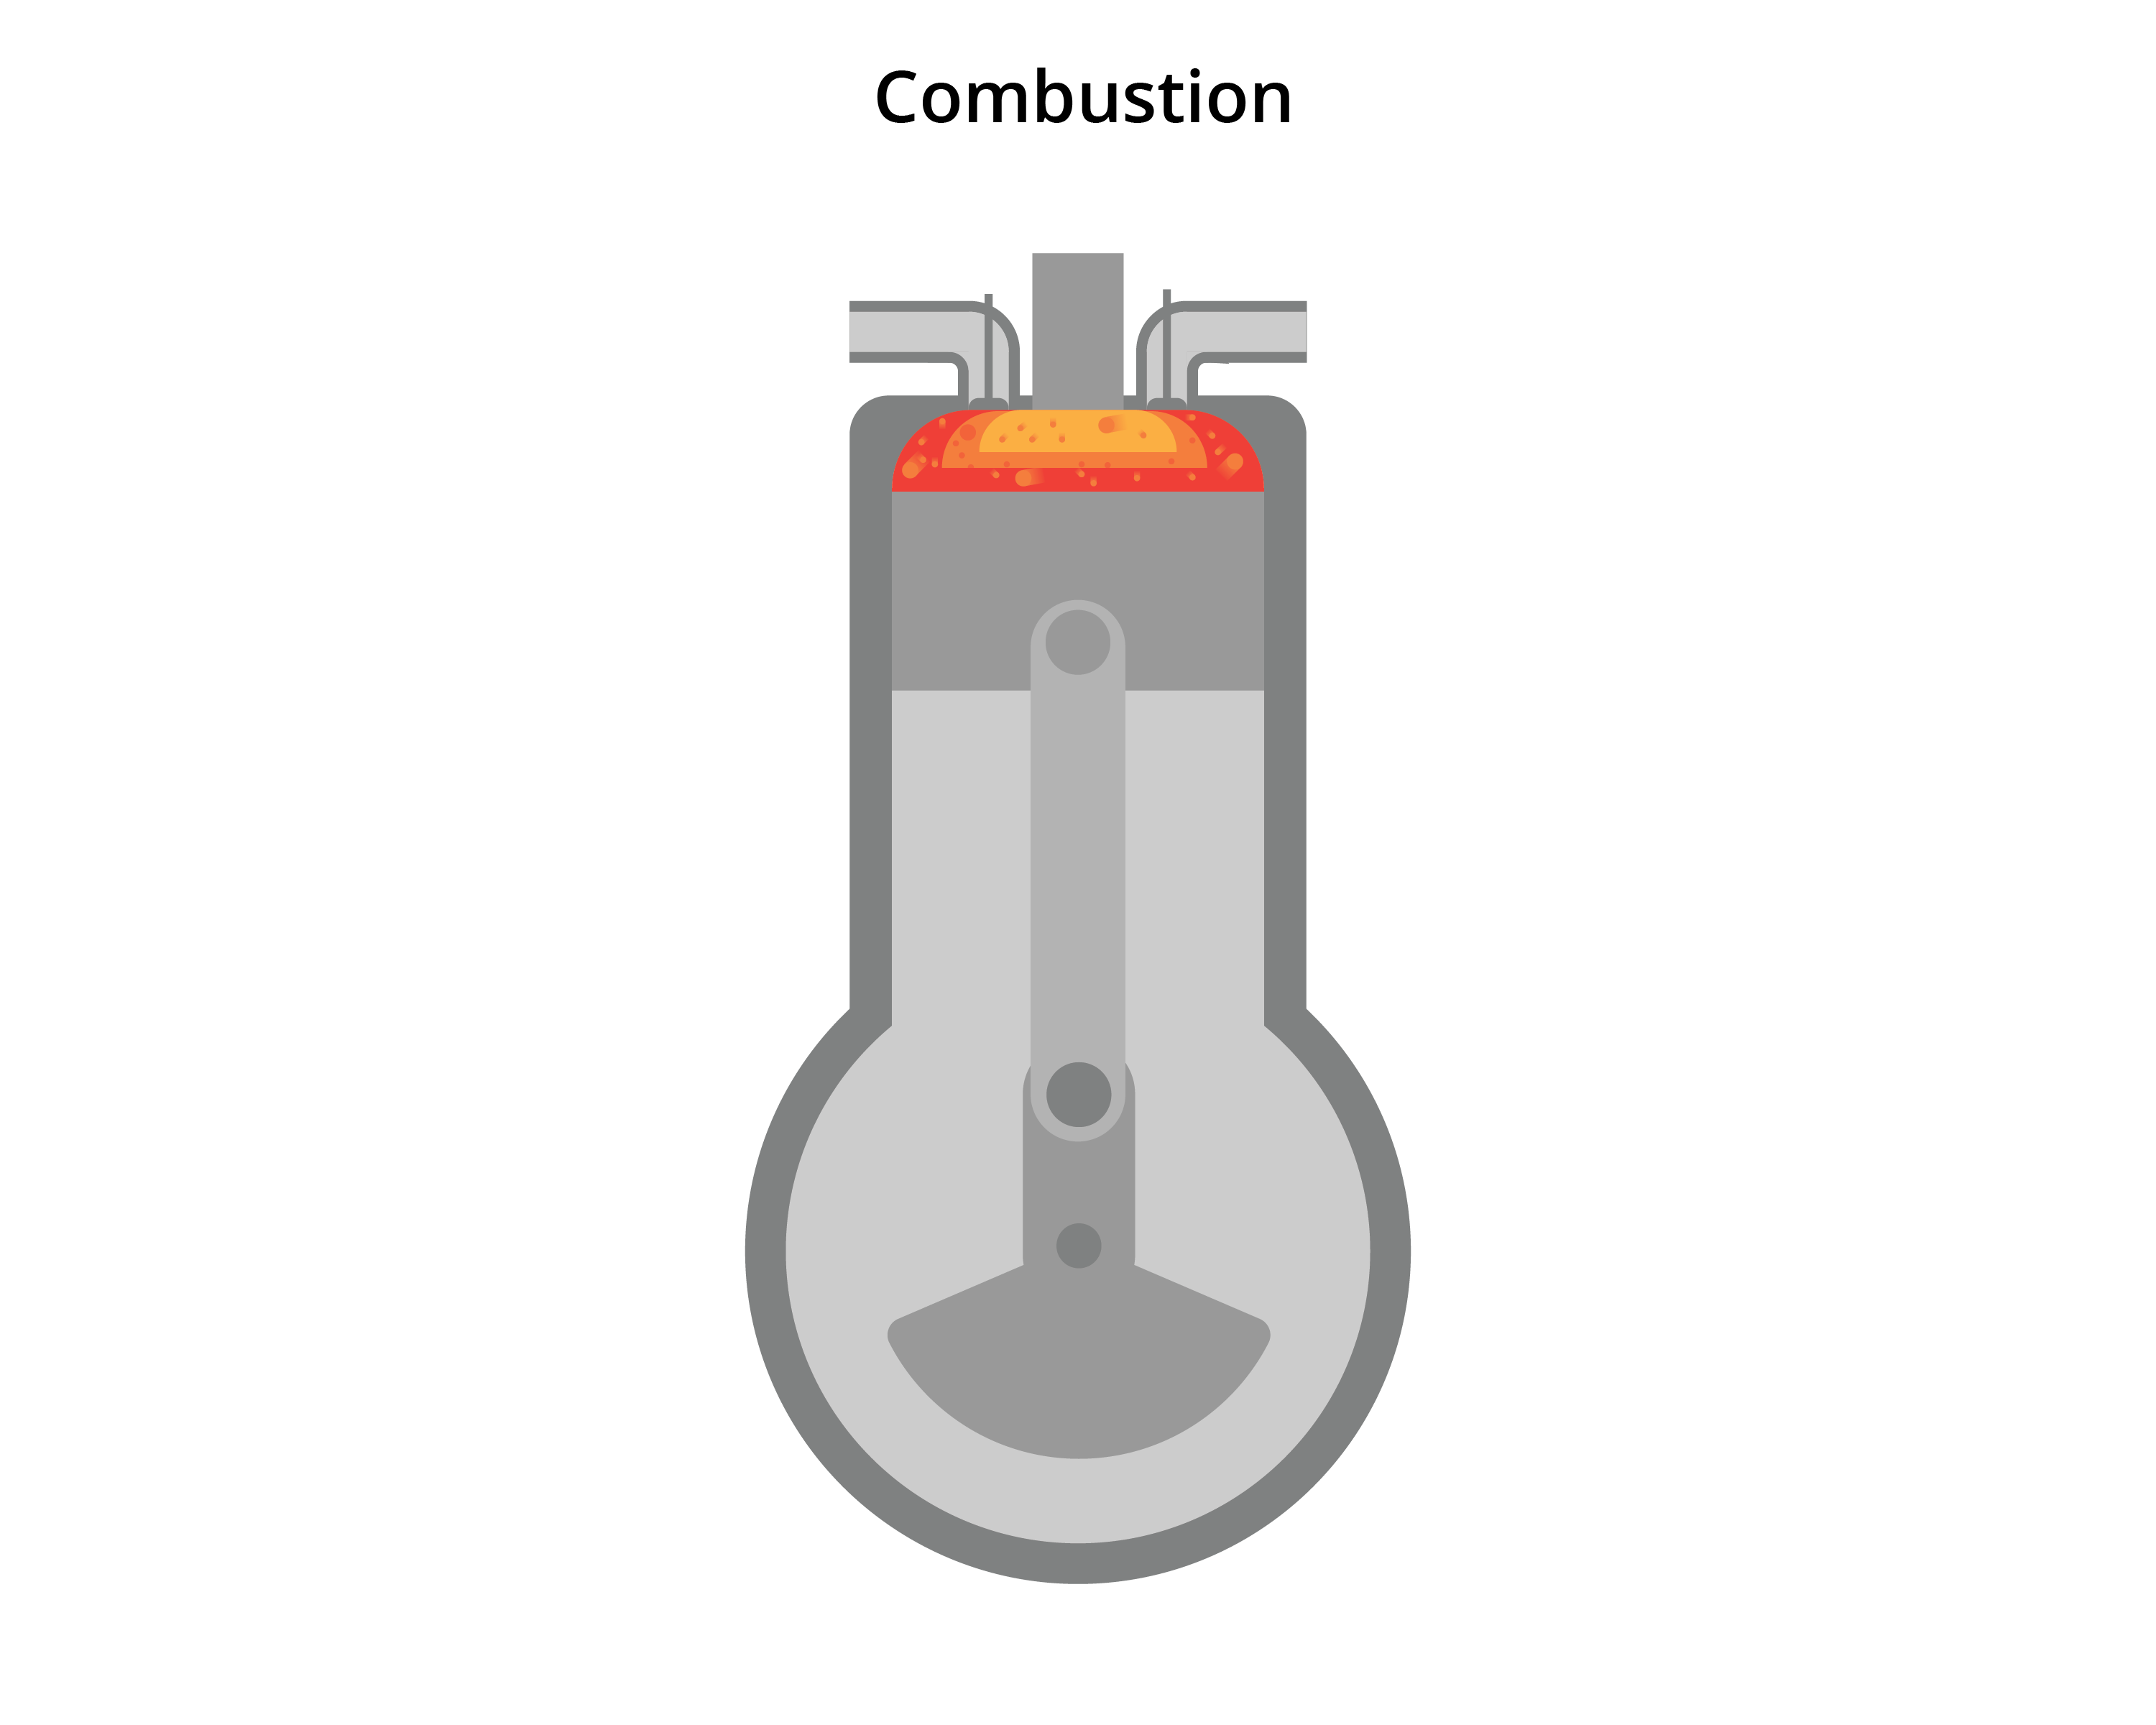
\includegraphics[width=0.75\textwidth]{engine-11.png}

\item There is now very high pressure inside the cylinder.  It pushes hard on the piston, which pushes the crank shaft.
\item When the piston reaches the bottom of this stroke,  the exhaust valve opens.
\item As the crank shaft pushes the piston up,  the carbon dioxide and water vapor is pushed out.

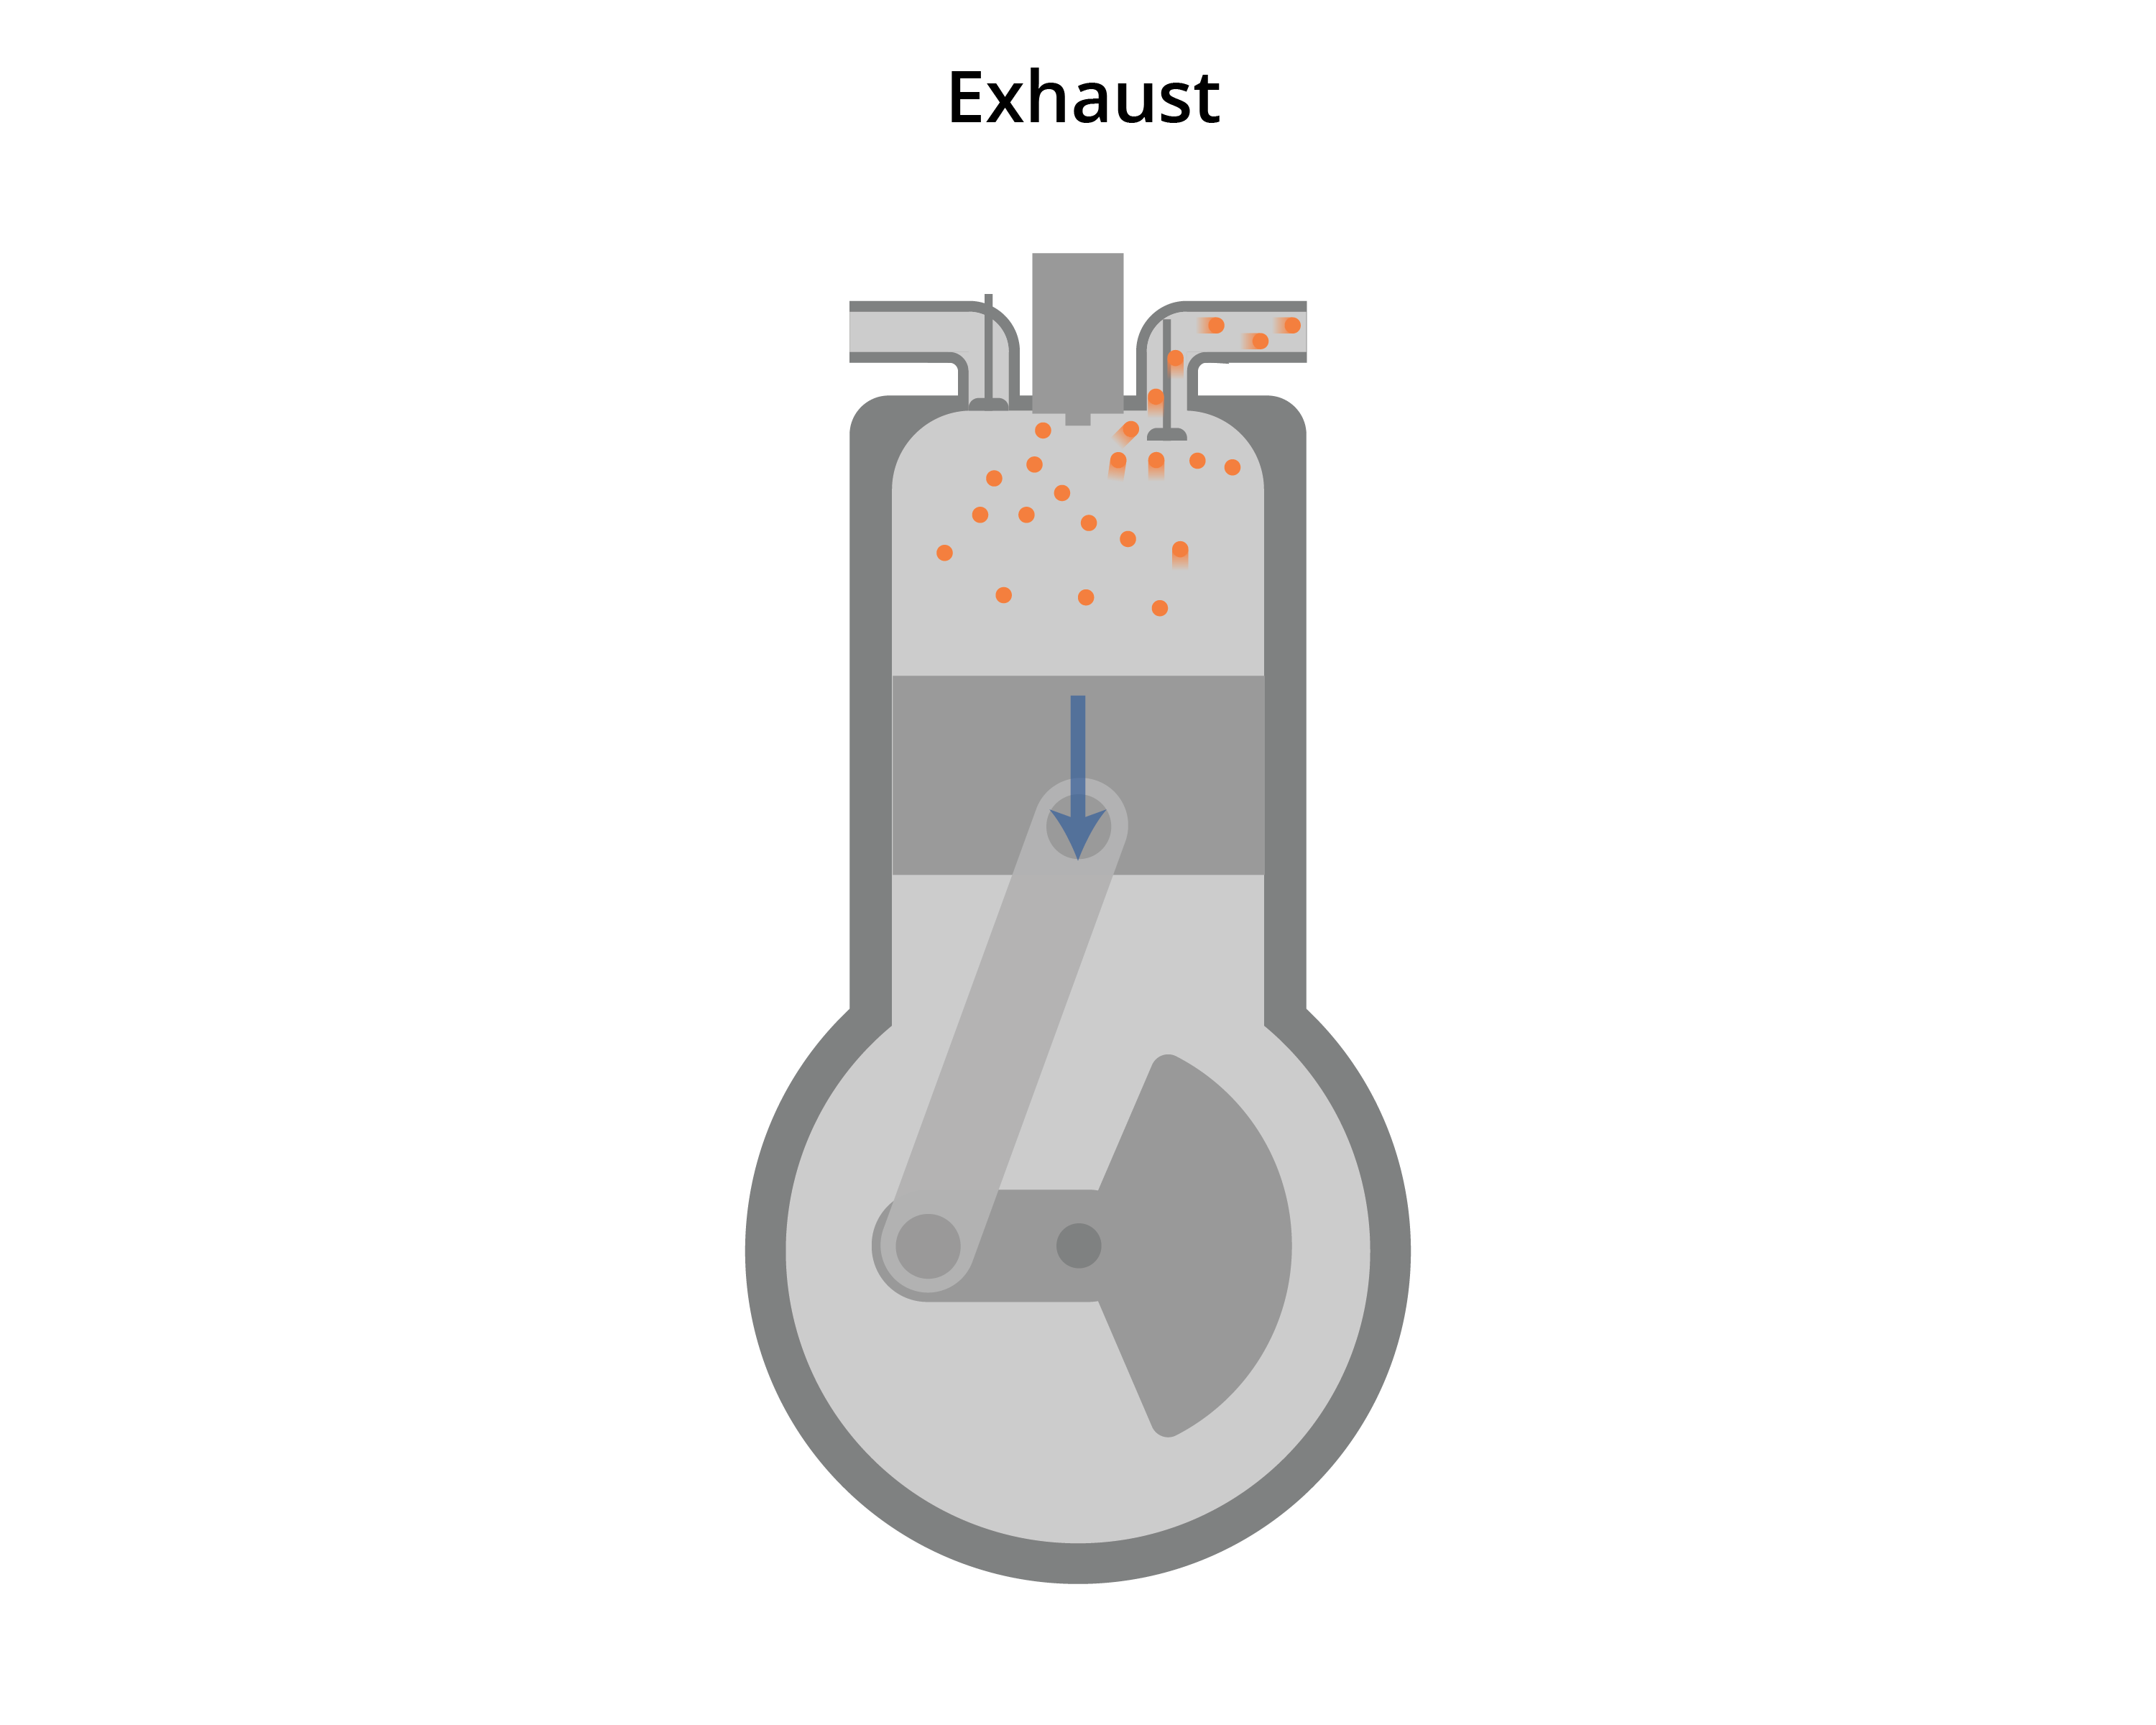
\includegraphics[width=0.75\textwidth]{engine-12.png}

\item When the piston reaches the top of this stroke,  the exhaust valve is closed.
\end{itemize}

\section{Dealing with Heat}

Burning fuel inside a block of metal generates a large amount of heat.  If there is too much heat,  parts of the engine will start to melt.  So, modern car engines are liquid cooled --- there are arteries in the engine block carrying a liquid (called "coolant").  The hot coolant is pumped through the radiator (where the air passing through takes away the heat), then back into the engine.

Note that the heat that is carried away by the coolant is wasted energy.    In fact,  of the total energy created in burning the fuel,  most car engines only transfer about 30\% to turning the crank shaft.  About 35\% of the heat goes out with the exhaust.  About 30\% is carried away by the coolant.  
The remaining waste (usually about  5\%) is lost to friction.

\section{Dealing with Friction}

From the description,  it is clear that there is a great deal of metal sliding against metal,  which would grind the engine up quickly if there were no lubrication.  In a modern car, the moving parts in the engine are constantly bathed in oil.  There is an oil pump that causes it to get sprayed on the crankshaft, the connecting rod, and in the cylinder under the piston (that is, not on the combustion side).  

The oil eventually falls through the oil into a pan at the bottom of the engine.   The oil pump sucks the oil up,  pushes it through a filter (so bits of metal are not pumped back into the engine),  and is then sprayed on the moving parts again.

\section{Challenges}

With a piston engine, there are a lot of things that can go wrong.  Let's enumerate a few:

\begin{itemize}

\item \textit{The seal around the piston leaks}.  Mechanics say "We aren't getting any compression."  The cylinder doesn't get much power to the drive train.

\item \textit{The valves open or the spark plug fires at the wrong time.}  This is known as a timing problem. 

\item \textit{The spark plug doesn't make a spark}. The spark plug has two prongs of metal and electrons jump from one to the other.  For a good spark,  the prongs need to be a very precise distance apart.  Sometimes you need to bend one of the prongs to get the right gap.  This is known as \newterm{gapping}.

\item \textit{The mix of fuel and oxygen is wrong.}  If there is too much fuel and not enough oxygen (so not all the fuel burns),  we say the mix is too rich.  If there is not enough fuel (so the pressure created by the burn is as high as possible), we say the mix is too lean.

\end{itemize}

\section{How We Measure Engines}

If you look up the specs on an engine,  you will see the following:

\begin{itemize}
\item The number of cylinders
\item The cylinder bore, which is the diameter of the cylinder
\item The piston stroke,  which is the distance the piston travels in the cylinder
\item The compression ratio,  which is the ratio between the maximum volume of the combustion change and the minimum volume of the combustion chamber
\item What fuel it runs on
\end{itemize}

The difference between the minimum and maximum value of the cylinder is known as its \newterm{displacement}. The displacement represents the volume of air/fuel sucked into the intake valve 
before the compression begins.

We often talk about the displacement of the entire engine, which the
 cylinder's displacement times the number of cylinders. The displacement of an engine can give you a
 good idea of how much power it can produce.
 
For motorcycles,  the displacement is often part of the name. For example,  the Kawasaki Ninja 650 has about 650 cubic centimeters of displacement.  

\section{The Ford Model T and Ethanol}

The Ford Model T was the first mass-produced car. It came out in 1908 and remained in production until 1927.  It had a four-cylinder engine that would run on ethanol, benzene, or kerosene.  For the purposes of this exercise, let's assume you are running yours on ethanol.

A molecule of ethanol has 2 carbon atoms, 6 hydrogen atoms, and 1 oxygen atom.  The oxygen in the atmosphere is $O_2$.   When one molecule of ethanol combines with 3 molecules of $O_2$,  2 molecules of $CO_2$ and 3 molecules of $H_2O$ are created.  A large amount of heat is also created --- 1330 kilojoules for every mole of ethanol burned.

The engine block is usually very hot once the engine has been running.  That is important because the ethanol will be completely vaporized at that temperature.

In any sample of air, 21 percent of the molecules will be $O_2$.

\begin{Exercise}[title={Fuel Mix for the Model T},  label=fuelmix]

On the Model T, a carburetor mixed the fuel and air before it went into the cylinder.   The question to answer in this exercise is: How rich should the mix be at sea level (100 kPa)?

On the Wikipedia page for the Model T,  we see the following facts:
\begin{itemize}
\item Cylinder bore: 9.525 cm
\item Piston stroke: 10.16 cm
\end{itemize}

You can assume that the air/fuel mixture is $80^\circ$ C before the pre-burn compression starts.  (Thus, the ethanol,  which boils at $78^\circ$ C, is in its vapor phase.)

The questions, then, are:

\begin{itemize}
\item What is the displacement of a single cylinder?
\item How many moles of gas ($80^\circ$ C and 100 kPa) will get sucked through the intake valve?
\item How many moles of vaporized ethanol should be part of that?
\item How many moles of $CO_2$  and  $H_2O$ are created in each burn?
\item How much heat is created in each burn?
\end{itemize}

(This exercise has a lot of steps, but nothing you don't already know.  You will need the ideal gas law to figure out how much many moles of air gets dragged into the cylinder.)

\end{Exercise}

\begin{Answer}[ref=fuelmix] 

The pre-compression temperature is $80\^circ \text{ C } + 273.15 = 353.15^\circ$ K.

The radius of the cylinder is $9.535/2 =4.7625$ cm.

The area of a cross section of the cylinder is $\pi r^2 = \pi (4.7625)^2 \approx 71.26$ ml.

So, the change in volume between the minimum and maximum volume is $ (71.26)(10.16) = 724$ ml, or 0.724 liters.

(With four cylinders,  the total displacement of a Model T is thus $ (4)(724) = 2,896$ cc.)

Now we use the ideal gas to figure out how many moles of gas will fit into 0.724 liters at 100 kPa and $353.15^\circ$ K.

$$n = \frac{PV}{rT} = \frac{(100)(0.724)}{(8.314)(353.15)} = 0.02466 \text{ moles of air+fuel }$$ 

So,  if we suck $n_a$ moles of air and $n_e$ moles of vaporized ethanol in to the cylinder:

$$n_a + n_e = 0.02466$$

So

$$n_a = 0.02466 -  n_e$$

21\% of $n_a$ is $O_2$:

$$n_{O_2} = 0.21 n_a = 0.21 (0.02466 -  n_e) = 0.005178 - 0.21 n_e$$

For a clean burn,  we need 3 times as many $O_2$ molecules as ethanol molecules.  Thus:

$$3 n_e  =   n_{O_2} = 0.005178 - 0.21 n_e$$

Solving for $n_e$:

$$n_e = \frac{0.005178}{3.21}  = 0.001613 \text{ moles  of ethanol}$$

For every molecule of ethanol that burns we get 2 molecules of $CO_2$: 0.003226 moles.

For every molecule of ethanl that burns we get 3 molecules of $H_2OI$: 0.004839 moles.

How much heat?  $(0.001613)(1330) =  2.145$ kilojoules from each burn.

\end{Answer}

\section{Compression Ratio}

Most of the inefficiency of a motor is heat that escapes through the exhaust valve.  If your piston stroke were long enough,  you could keep increasing the volume (which would cool the gases inside) until the gases inside were the same temperature as the outside world.  Then there would be no wasted heat in the exhaust.

For this reason, generally,  engines with a higher compression ratios tend to waste less energy through the heat of the exhaust.  The Model T had a compression ratio close to 4:1.  Modern car engines typically have compression ratios between to 8:1 and 12:1.  

Cars with especially high compression ratios often require fuels with a lot of kilojoules per mole --- we say \newterm{high octane}.   If the fuel does not have enough energy,  the engine makes loud knocking noises, as the pistons do not have enough energy to push through their entire stroke.

It turned out that an easy way to boost the octane of the gasoline was to add a chemical called tetraethyl lead.  Gasoline containing tetraethyl lead was known at "Leaded Gasoline", and was intended to prevent the knocking.   It is difficult to overstate the damages caused by putting large amounts of lead in the air.  Gradually, starting with Japan in 1986, every country in the world has banned leaded gasoline.

\section{The Choke and Direct Fuel Injection}

Most cars built before 1990 will have a carburetor,  which ensures that the ratio between fuel and oxygen is constant, regardless of the amount of fuel released by the throttle.   

If you go to start an old car on a cold morning,  the cold engine will not vaporize the fuel properly, and the engine may not have enough power to start.   For this reason,  most carburetors have a \newterm{choke value} that makes the mix richer.  (If you pull the choke valve,  be sure to push it back after the engine warms up.)

The carburetor was a common source of engine problems and inefficiencies.   Starting in the 1990s,  car engines started using direct fuel injection. Air still came in through the intake manifold,  but fuel was sprayed directly into the cylinder by a fuel injection system.

In modern cars,  the fuel injection system is controlled by a computer (an  \newterm {Engine Control Module} or ECM), which delivers the fuel at the perfect time with the perfect amount based on environmental variables like the temperature of the engine and the barometric pressure (usually related to that altitude at which the engine is operating).


